\documentclass{article}

% Language setting
\usepackage[english]{babel}

% Set page size and margins
\usepackage[letterpaper,top=2cm,bottom=2cm,left=3cm,right=3cm,marginparwidth=1.75cm]{geometry}

% Useful packages
\usepackage{amsmath}
\usepackage{graphicx}

\usepackage[colorlinks=true, allcolors=blue]{hyperref}
\usepackage{float}
\DeclareMathOperator*{\argminA}{arg\,min}

\title{CS461 HW 4}
\author{John Bailon (jlb671), Patrick Bailon (plb103)}
\date{December 13, 2024}

\begin{document}
\maketitle

\noindent
Submission Files:

Le\_Net5\_1.pt

Le\_Net5\_2.pt

Distort Images.py

RBF.py

LeNet5\_1.py    

LeNet5\_2.py

test1.py 

test2.py 

Model Link: https://rutgers.box.com/s/3l309sfm19va715rt8uabmxiztdma5gi

\section{LeNet5 Implementation}
\subsection{Architecture}
Following the architecture from LeNet5, our model goes contains 3 convolution layers, 2 average pooling layers, and 2 fully connected layers. A tanh activation function is used after each pooling layer. For the RBF implementation, we used the DIGITS dataset. For each digit, we took all the images of that digit, processed it with max-pooling with kernel size 8 and stride of 8, averaged them all together, then resized it to 7x12 as required. These bitmaps were then flattened and stacked with the other bitmaps. The resulting matrix was 10x84 and was used in the final layer of our model. This layer find the Euclidean distance between the input and each row vector in our matrix as outlined in equation (7) in the paper.

\subsection{Training}
In the submission includes both models and test codes as well as the RB matrix, which is needed for the the first model to work.

\subsection{Performance Evaluation}
After 20 iterations the model achieved a 96\% accuracy on the test set. We noticed during training that error would fluxate rapidly after 3-4 iterations when the learning rate was set to 0.0001, leading us to settle with a learning rate of 0.000001.\\~\\The confusion matrix is given as follow:
$$
\begin{bmatrix}
973&0&2&1&1&2&6&0&6&3\\
0&1118&1&0&1&0&3&11&1&7\\
0&2&1001&2&0&0&0&26&3&0\\
0&8&9&988&0&18&0&8&7&8\\
0&0&1&0&944&0&3&0&2&6\\
1&1&0&5&0&853&6&1&2&1\\
3&1&0&0&5&11&937&0&10&2\\
0&0&12&8&0&1&0&974&3&4\\
2&4&3&5&1&5&3&1&928&12\\
1&1&3&1&30&2&0&7&12&966\\
\end{bmatrix}
$$
Where the rows represent the predicted digit and the columns represent the target digit.\\~\\{\centering
   {
\includegraphics[width=0.24\textwidth]{0.png}} 
   {
\includegraphics[width=0.24\textwidth]{1.png}} 
    {
\includegraphics[width=0.24\textwidth]{2.png}}
    {
\includegraphics[width=0.24\textwidth]{3.png}}
    {
\includegraphics[width=0.24\textwidth]{4.png}}
      {
\includegraphics[width=0.24\textwidth]{5.png}}
        {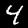
\includegraphics[width=0.24\textwidth]{6.png}}
          {
\includegraphics[width=0.24\textwidth]{7.png}}
            {
\includegraphics[width=0.24\textwidth]{8.png}}
              {
\includegraphics[width=0.24\textwidth]{9.png}}\\
              Misclassified digits in order. Here the first image is of a digit the model classified as 0, In the second the model predicted as 1 and so on.\\~\\
    \label{fig:foobar}
    {\includegraphics[width=0.85\textwidth]{Figure_1.png}}\\
    Test error(orange) and Train error(blue)}
    
\section{Modifying LeNet5 to Handle Unseen Data}
\subsection{Planning a New Model}
To address unseen data we first need to create a new test set. We selected a subset of the original training set and applied various transformations to it. Specifically, we used Pytorch's RandomPerspective and RandomRotation functions with a distortion scale of 0.6 and rotation angle of 0 to 45, respectively. The new data set now has images that are not centered and rotated various amounts.

Next, we retested the original model with this new data set. The test accuracy tanked considerably. It's accuracy was 65\% and generated the following confusion matrix: 
$$
\begin{bmatrix}
597&0&4&2&2&3&15&5&6&7\\
33&1068&83&132&183&66&115&212&110&168\\
1&16&613&31&19&5&4&24&6&5\\
2&34&73&612&8&30&6&37&26&3\\
9&2&13&1&541&0&112&9&25&8\\
70&5&25&76&11&594&51&24&59&40\\
18&0&4&1&24&92&561&0&25&4\\
0&8&152&62&15&18&1&654&14&20\\
14&2&26&31&24&14&8&4&522&8\\
236&0&39&62&155&70&85&59&181&746\\
\end{bmatrix}
$$

We can see that the model isn't robust against transformations within the image. 

To start, we made relatively simple modifications to the current architecture. ReLU replaced Tanh activation functions as ReLu offers performance benefits, such as a simpler derivative, and allows expression of greater positive or extreme values. We also switched max pooling instead of average pooling as max pooling will help select more prominent features. 

Additionally, we added more regularization control by adding Batch norm and dropout functions in each of the convolutional layers. In experimenting with dropout values, we found that higher values like 0.3 negatively affected the model's performance and settled with a dropout value of 0.1. We also opted to use Pytorch's built-in Pytorch Adam optimizer instead of our simple gradient descent optimizer to handle bias correction and noisy gradients.

Lastly, we looked to implement the spatial transformer network. Given that most of the transformations between the regular MNIST data set and the distorted data set were stretch/shrink and rotations, it made sense to add a spatial transformer to help correct these transformations. We constructed a localization network similar to the first convolutional layer and then used the torch functional library to fix and sample the generated grid.

With these changes, we trained the new model on the original MNIST data set then tested it on the original and distorted test set.

On the original set, it had 97.91\% accuracy and generated the following confusion matrix
$$
\begin{bmatrix}
 964&    0&    2&    0&    0&    0&    6&    0&    4&    2\\
   0& 1113&    0&    0&    0&    0&    5&    2&    0&    0\\
  10&    2& 1026&    3&    1&    1&    2&    8&    1&    1\\
   0&    2&    1&  999&    0&    4&    1&    3&    3&    5\\
   0&    0&    0&    0&  950&    1&    4&    1&    1&    7\\
   1&    1&    0&    5&    1&  881&    6&    0&    6&   14\\
   3&    1&    0&    0&    1&    2&  930&    1&    2&    0\\
   1&    3&    2&    2&    1&    2&    0& 1011&    1&    8\\
   1&   13&    1&    1&    2&    1&    4&    0&  955&   10\\
   0&    0&    0&    0&   26&    0&    0&    2&    1&  962\\
\end{bmatrix}
$$


On the distorted set, it had 75.11\% accuracy and generated the following confusion matrix:

$$
\begin{bmatrix}
685&   0&   1&   7&   1&   7&  10&  11&  18&  26\\
  2& 858&   3&  16&  42&   2&   9&   6&  21&  27\\
 34& 134& 876&  74&  65&  12&  51&  67&  76&  20\\
  2&   3&  38& 740&  10&  16&   4&  31&  25&  13\\
  5&  12&  23&  13& 736&   6& 110&  18&  25&  23\\
 35&  26&   6&  58&  14& 731&  56&  32&  64&  53\\
 73&  13&  12&   2&   5&  70& 654&  15&  52&  21\\
  3&  57&  50&  48&  38&   9&   2& 826&  23&  40\\
 17&  24&   8&   3&  19&   6&  14&   7& 628&   9\\
124&   8&  15&  49&  52&  33&  48&  15&  42& 777\\
 \end{bmatrix}
$$

\end{document}